\chapter{Implementierung}\label{implementierung}

\todo{einleitung schreiben}
%Für unsere Implementation wird für das Zwischenspeichern von Daten ein Serviceworker eingesetzt. Serviceworker können wie ein Proxy zwischen dem Webbrowser und dem Webserver agieren, welcher die Webseite bereitstellt. Stellt ein Browser eine Anfrage, so wird diese vom Serviceworker abgefangen. Der Serviceworker schaut zunächst in seinem Cache, der sog. IndexDB, ob er die gestellte Anfrage beantworten kann. Ist dies nicht der Fall, so wird die Anfrage an den Webserver weitergeleitet. Wird die gleiche Anfrage nochmals gestellt, kann diese aus dem Cache beantwortet werden, da gestellte Anfragen eine gewisse Zeit lang zwischengespeichert werden.
%\begin{figure}[!h]
%	\centering
%	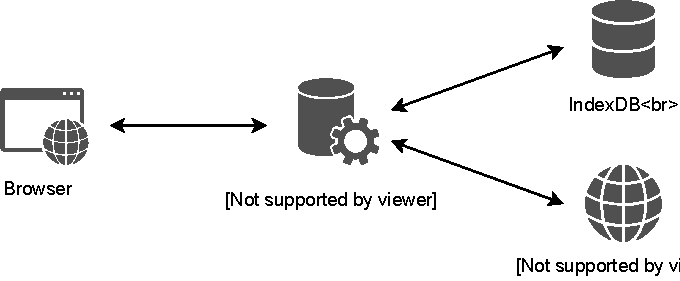
\includegraphics[width=0.8\textwidth]{figures/ServiceWorker}
%	\caption[A Figure Short-Title]{A Figure Title}
%	\label{fig:sequenceDiagram}
%\end{figure}
%
%
%Die von uns eingesetzte Technologie zur Übertragung von Daten zwischen Browsern ist WebRTC. WebRTC ist ein offener Standard und ermöglicht es Browser paarweise zwecks Datenaustausch zu verbinden. Der große Vorteil dieser Technologie ist, dass sie direkt von modernen Browsern unterstützt wird, wodurch keine zusätzliche Software installiert werden muss. Konkret wird von uns ein sog. DataChannel genutzt.
%
%Für den Datenaustausch müssen wechselseitig DataChannel zueinander aufgebaut werden. Die Ausgangslage ist, dass die Schüler wissen, dass es den anderen gibt, aber nicht wie der jeweils andere zu erreichen ist. Um diese Problematik zu lösen, existiert ein Vermittlungsserver (Signaling server).
%
%Als erstes werden Informationen, über die Verbindung die aufgebaut werden soll, an den Signaling server gesendet. Technisch wird ein SDP-offer gesendet, wobei SDP für Session Description Protocol steht. Dieses SDP-offer leitet der Signaling server an die Schüler in der Klasse/Schule weiter. Geantwortet wird mit einer SDP-answere, welche Informationen über die abgestimmte Verbindung enthält und über den Signaling server zurück geleitet wird.
%
%Damit eine direkte Verbindung aufgebaut werden kann, müssen über den Signaling server noch weitere Informationen wie ICE-Kandidaten ausgetauscht werden. ICE steht hierbei für Interactive Conectivity Establishment und ist fester Bestandteil von WebRTC. Es ist für den Aufbau der Browser-zu-Browser-Verbindung verantwortlich. ICE-Kandidaten enthalten hauptsächlich Informationen darüber wie ein bestimmter Nutzer erreichbar ist (also z.B. private oder öffentliche IP-Adresse). Ermittelt werden diese ICE-Kandidaten mithilfe eines STUN-Servers und dem dazugehörigen Session Traversal Utilities for NAT (STUN) Protokoll. Wie der Name des Protokolls schon verrät, wird es vor allem benötigt um auch Nutzer erreichen zu können die keine eigene öffentliche IP-Adresse besitzen, bei denen also Network address translation (NAT) eingesetzt wird. Dies ist aufgrund der mangelnden Anzahl an IPv4-Adressen bei fast jedem Internetnutzer der Fall.
%
%In dem Signaling server selbst wird die Logik abgebildet, wie die Klassen und Schüler miteinander in Verbindung stehen. Implementiert wurde dieser mit socket.io, da die native Klassenorganisation und Websocket-Technologie sich nahezu perfekt für unser Szenario anbot.

\section{Technologiewahl}
Das \pTp \cdn ist eine Javascript Bibliothek, die nach erfolgreicher Einbindung und Konfiguration im Hintergrund eigenständig läuft. Es werden zwei Javascript Dateien zur Verfügung gestellt. Das Service Worker Script, und das \pTp \cdn Client Script. Beide Scripte müssen von der Anwendung eingebunden werden. Der Server muss einen Faye Websocket Server bereit stellen. Da das Peer Meshing über die Konfiguration des Faye Channels geschieht muss der Server gegebenefalls eine Peer Meshing Strategie implementieren. Zur einfacheren Einbindung in bestehende Projekte wird ein NodeJS Modul so wie ein Ruby Gem bereit gestellt. Das Ruby Gem bindet das ServiceWorker Script im Public Ordner der Ruby-on-Rails Anwendung ein und das \pTp CDN Script im vendor/assets Ordner.

Der Javascript Code ist in ES6 geschrieben und wird mittels Babel\footnote{https://babeljs.io/} in Browser kompatiblen Javascript Code übersetzt und anschließend mit Node-minify komprimiert. \footnote{https://www.npmjs.com/package/node-minify}

\section{Architektur}
\todo{einleitung schreiben}

\begin{figure}[!h]
	\centering
	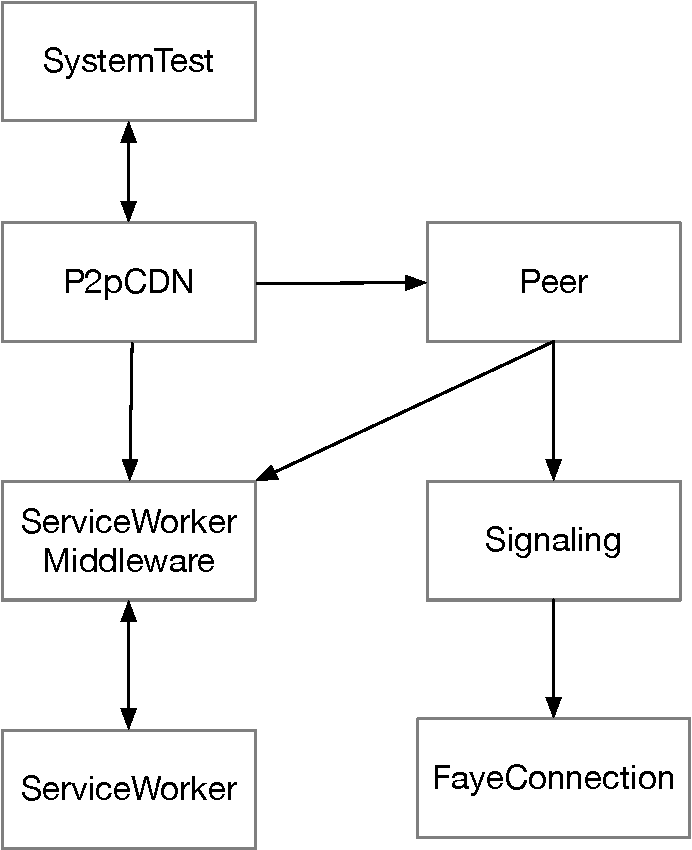
\includegraphics[width=0.8\textwidth]{figures/Klassendiagramm}
	\caption[A Figure Short-Title]{Klassendiagramm}
	\label{fig:Klassendiagramm}
\end{figure}

\subsection{Client Script}

Das Javascript Plugin besteht aus sieben Komponenten. Die Klasse P2pCDN bildet die Schnittstelle nach außen und stellt Funktionalitäten zum initialisieren und konfigurieren des \cdns bereit. Außerdem macht es den SystemTest nach außen verfügbar. P2pCDN nimmt die Konfiguration entgegen und initialisiert ein Peer Objekt. Das Peer Objekt repräsentiert den eigenen \client in dem \pTp Netzwerk. Es hält den eigenen Zustand und verwaltet die Verbindungen anderen \clients und verwaltet deren Ressourcen Hashes. Das Peer Objekt nutzt Funktionalitäten des Signaling Moduls um Verbindungen zu anderen \clients aufzunehmen. Das Signaling Modul implementiert das Webrtc Signaling Protokoll. FayeConnection abstrahiert die beim Signaling verwendete Websocket Bibliothek, in diesem Fall Faye um es zu ermöglichen auch andere Websocket Bibliotheken zu verwenden.
Die ServiceWorker Middleware fungiert als Vermittler zwischen Service Worker und Client Script und ist für die Initialisierung des Service Workers zuständig. Die Komponente arbeitet Event basiert und registriert sich auf folgende Events:
\begin{description}
	\item[peer:onRequestResource]\hfill \\
	Wird von der Serviceworker Middleware ausgelöst wenn der Service Worker eine Ressource über das \pTp CDN anfragt. Der Peer registriert auf dem Event und bearbeitet die Anfrage.
	\item[peer:onAddedResource / peer:onRemovedResource]\hfill \\
	Speichert der Service Worker eine Ressource so teilt er dies der ServiceWorker Middleware über einen Message Channel mit. Diese löst anschließend das peer:onAddedResource Event aus um dem Peer über die Änderung zu informieren, der die das Update an die verbundenen \clients weiter leitet.
	\item[sw:onRequestCache]\hfill \\
	Stellt der Peer eine neue Verbindung zu einem anderen \client her so sendet er eine Liste seiner gespeicherten Ressourcen an den Client. Diese Liste wird vom Service Worker verwaltet. Um an den Inhalt seines Caches zu kommen sendet der Peer das sw:onRequestCache Event mit einem Callback der bei erfolg ausgeführt wird. Die ServiceWorker Middleware leitet die anfrage über den Message Channel an den Service Worker weiter.
%	\item[Message events vom Service Worker]\hfill \\
%	
%\end{description}
%
%\begin{itemize}
%	\item heartbeats
%\end{itemize}

\subsection{Service worker}

\begin{figure}[!h]
	\centering
	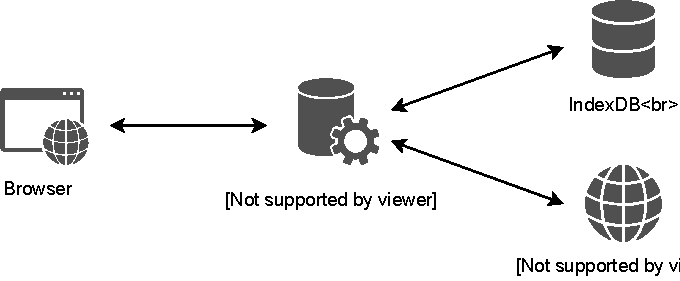
\includegraphics[width=0.8\textwidth]{figures/ServiceWorker}
	\caption[A Figure Short-Title]{Service Worker}
	\label{fig:serviceWorker}
\end{figure}
\todo{diagram fixen}

Als Proxy zwischen Client Anwendung und Browser wird ein Service Worker verwendet. Der Service Worker fängt von der Anwendung gesendete Anfragen im Fetch event ab und versucht sie als erstes durch den eigenen Cache zu beantworten. Ist die Anfrage nicht bereits im Cache vorhanden wird versucht sie über das \pTp Netzwerk zu laden. Ist das nicht möglich so lädt er sie vom Server. 
Um eine Anfrage über das \pTp Netzwerk zu beantworten muss zuvor das Client Script geladen sein, da Service Worker die Webrtc API nicht unterstützen. Die Kommunikation zwischen Service Worker und Anwendungs Script geschieht mit Hilfe der post Message API\footnote{https://developer.mozilla.org/en-US/docs/Web/API/Window/postMessage}. Um sicherzustellen das das Client Script geladen und bereit zur Kommunikation ist sendet der Service Worker eine nicht blockende Heartbeat Anfrage an das Script. Antwortet das Script nicht innerhalb eines bestimmten Zeitfensters so muss der Service Worker davon ausgehen, dass es noch nicht geladen ist. Die Anfrage wird an den Server weiter geleitet. Da nicht davon ausgegangen werden kann das das Script verfügbar bleibt nachdem es geladen wurde, die Seite könnte z.B. geschlossen worden sein, muss der Service Worker sich vor jeder Blockenden Anfrage vergewissern das das Script in der Lage ist zu antworten.
Nachrichten die zwischen Anwendungs Script und Service Worker gesendet werden haben das Format: { type: "Art der Nachricht", msg: "Inhalt der Nachricht" }. Das Attribut "type" kann folgende werde enthalten: "resource", "cache", "hearbeat". Nachrichten vom Typ "resource" ordnen den Service Worker an eine Nachricht aus seinem Cache an das Anwendungs Script zu übergeben. Empfangt der Service Worker eine solche Nachricht lädt er die Angefragte Ressource aus dem Cache und fügt sie der Antwort bei. Nachrichten vom Typ "cache" dienen dazu beim Server den momentanen Inhalt des caches zu erfragen. Dies wird genutzt um einem neu Verbundenen Peer die Liste der aktuell gecachten Ressourcen mitzuteilen. Mit dem Typ "heartbeat" erfragt der Service Worker beim Anwendungs Script ob es momentan verfügbar ist.   
Ist das Script noch nicht verfügbar hat der Service Worker zwei Möglichkeiten damit umzugehen. Er kann darauf warten das das Script verfügbar ist und alle Anfragen bis dahin aufhalten oder er leitet die Anfragen direkt an den Server weiter. Leitet er die Anfragen direkt an den Server so wird die Ladezeit der Ressource nicht verzögert, jedoch ist es erst Möglich Ressourcen über das \pTp \cdn zu laden wenn das Script geladen wurde. Das \cdn arbeitet weniger effektiv, dafür wird das Nutzererlebnis jedoch nicht negativ beeinflusst. Wartet der Service Worker bis das Script aktiv ist, so können mehr Anfragen über das \cdn beantwortet werden, jedoch ist nicht garantiert wann es antwortet oder ob es überhaupt fehlerfrei geladen wird. Deshalb wurde sich bei der Implementierung des \cdns dafür entschieden das in diesem Fall Anfragen direkt an den Server weiter geleitet werden sollen. Das hat zur Folge das sich die gewählte Implementierung besonders für Single Page Applications sowie für Anwendungen die Navigationen z.B. mithilfe von Turbolinks vermeiden eignet. Bleibt beim Laden von neuen Inhalten das Anwendungsscript in Ausführung und muss nicht geladen werden, so kann der Service Worker Anfragen über das \pTp Netzwerk beantworten.
 Vor der Registrierung des Service Workers speichert das Anwendungs Script die Konfiguration in die IndexDB des Browsers. Der Service Worker liest die Konfiguration von dort aus. Auf diesem Weg ist es möglich den Service Worker dynamisch zu konfigurieren und ihm unter anderem die zu verarbeitenden URLs zu übergeben. Die URLs werden als Regex übergeben. Fällt eine Anfrage nicht in die übergebenen URLs so unterbricht er die Verarbeitung und die Anfrage wird vom Server beantwortet.
 Sobald der Service Worker aktiv ist ist ruft er self.clients.claim() auf um Sicherzustellen das er schon beim ersten Seitenaufruf aktiv ist und anfragen der Clients verarbeiten kann.
 
\section{Signaling Server}
Der Signaling Server nutzt Faye\footnote{https://faye.jcoglan.com/ruby/websockets.html} als Websocket Bibliothek. Die Anwendung muss lediglich einen Faye Server anbieten um das Signaling zu ermöglichen. Der Verbindungsaufbau wird im Anschluss Client seitig gehandhabt. 
Um Clients den Peer Meshes zuzuordnen werden verschiedene Websocket Channels verwendet. Wird zwei Clients der selbe Datachannel in der Konfiguration übergeben so befinden sie sich im selben Peer Mesh. So ist eine einfache Konfiguration möglich. Das \cdn selbst macht keine Annahmen darüber welche Clients sich sinnvollerweise im selben Mesh befinden sollten. Die Entscheidung darüber ist der Anwendungslogik überlassen. Dadurch ist es möglich ein Domänen spezifisches Peer Meshing vorzunehmen.

%\begin{itemize}
%  \item websockets faye
%  \item gleicher data channel zur Bildung von meshs
%  \item ID pro client
%  \item max id length muss festgelegt werden für chunking
%  \item Protokoll von P2PCDN umgesetzt
%  \item Protokoll erklären
%  \item Diagram Protokoll
%  \item Peer Meshing wird von anwendung übernommen
%\end{itemize}

\subsection{Slidesync}
Um das Signaling zu realisieren implementiert Slidesync ein eigene Klasse die für die Zuordnung von \clients zu Peer Meshes verantwortlich ist. Der Klasse wird der Scope des Aufrufs so wie die maximale Mesh Größe bei der Initialisierung übergeben. Wobei der Scope die ID des aufgerufenen Events ist. Durch Aufruf der join() Methode wird der Peer einem geeigneten Mesh zugeordnet und der Faye Channel des Meshes zurückgegeben. Dabei wird immer das erste freie Mesh gewählt um möglichst viele volle Meshes zu erreichen. 
Die Zuordnung muss performant geschehen und in einem scalierten Multi Server Setup funktionieren. Um dies zu erreichen wird Redis als Datenspeicher verwendet. Redis bietet geeignete Datenstrukturen mit geringen Zugriffszeiten und ist gut für ein multi Server Setup geeignet. 
Die Klasse speichert die liste der verfügbaren Submeshes in einer Liste. Jedes Mesh wird über eine Aufsteigende ID in Kombination mit dem Scope identifiziert. Mit Hilfe eines Redis Counters wird die ID des letzten Submeshes gespeichert. Dadurch lassen sich alle angelegten Meshes ermitteln ohne sie explizit speichern zu müssen. Erreicht ein Mesh die Maximale Teilnehmerzahl so wird es aus der Liste der verfügbaren Submeshes entfernt. Ist kein freies Mesh verfügbar so wird ein neues Mesh eröffnet. Dazu wird der Counter der letzten Mesh ID erhöht und ein neues Mesh mit dieser ID wird der Liste der verfügbaren Meshes hinzugefügt. Im Anschluss wird ein Hintergrund Job gestartet der überprüft ob bereits angelegte Meshes wieder frei geworden sind. Dazu wird für jedes Mesh überprüft ob sich alle Teilnehmer in der letzten Minute zurückgemeldet haben. Haben sich Teilnehmer nicht zurück gemeldet, so wird das Mesh wieder zu den verfügbaren meshes hinzugefügt. Da über sämtliche Submeshes und alle Peers iteriert werden muss macht es Sinn die Operation im Hintergrund durchzuführen.
Die Zuordnung von Teilnehmern zu Meshes wird für jedes Mesh ein Redis Set angelegt in dem die ID jedes Peers der dem Mesh beigetreten ist gespeichert wird. Zusätzlich wird für jeden Peer ein temporärer Key angelegt der nach 40 Sekunden automatisch gelöscht wird. Um Statistiken über Events zu erheben meldet sich jeder Teilnehmer eines Events alle 30 Sekunden bei dem Server und übermittelt Daten von seinem Client. Im Rahmen dieser Statistischen Erhebung wird ebenfalls der temporäre key erneuert, falls er sich am \pTp Netzwerk beteiligen kann. Ist der temporäre Key für einen Peer nicht verfügbar so wird angenommen das er nicht mehr am \pTp Netzwerk teilnimmt und sich demnach auch nicht mehr in dem Peer mesh befindet.     

\subsection{\schulCloud}

Die Schul-Cloud stellt ebenfalls einen Faye Server bereit über den das Signaling gehandhabt wird. Als Scope für die Peer Meshes wird die Schulklasse der Schüler verwendet. Da Schulklassen nur eine begrenzte Größe haben ist eine Unterteilung nicht notwendig.


\section{Client UI Event}
Um es der einbindenden Anwendung zu ermöglichen auf Änderungen bezüglich der verbundenen Peers sowie deren Ressourcen zu Reagieren stellt das Plugin das Event ui:onUpdate bereit das bei Änderungen ausgelöst wird. Das Event übergibt das Peer Object des Clients wodurch der Event Empfänger zugriff auf die Anzahl der verbundenen Peers so wie deren Ressourcen hat. 

\section{Nachrichten protocol}

Für die Funktion des \cdns sind einige Nachrichten zwischen den Komponenten und den Clients notwendig. Im Folgenden wird auf einige dieser Nachrichten genauer eingegangen, sowie der Kommunikationsablauf zweier \clients anhand eines Beispiels erläutert.

\subsection{Beispielhafter Kommunikationsfluss zwischen zwei Clients}
\begin{figure}[!h]
	\centering
	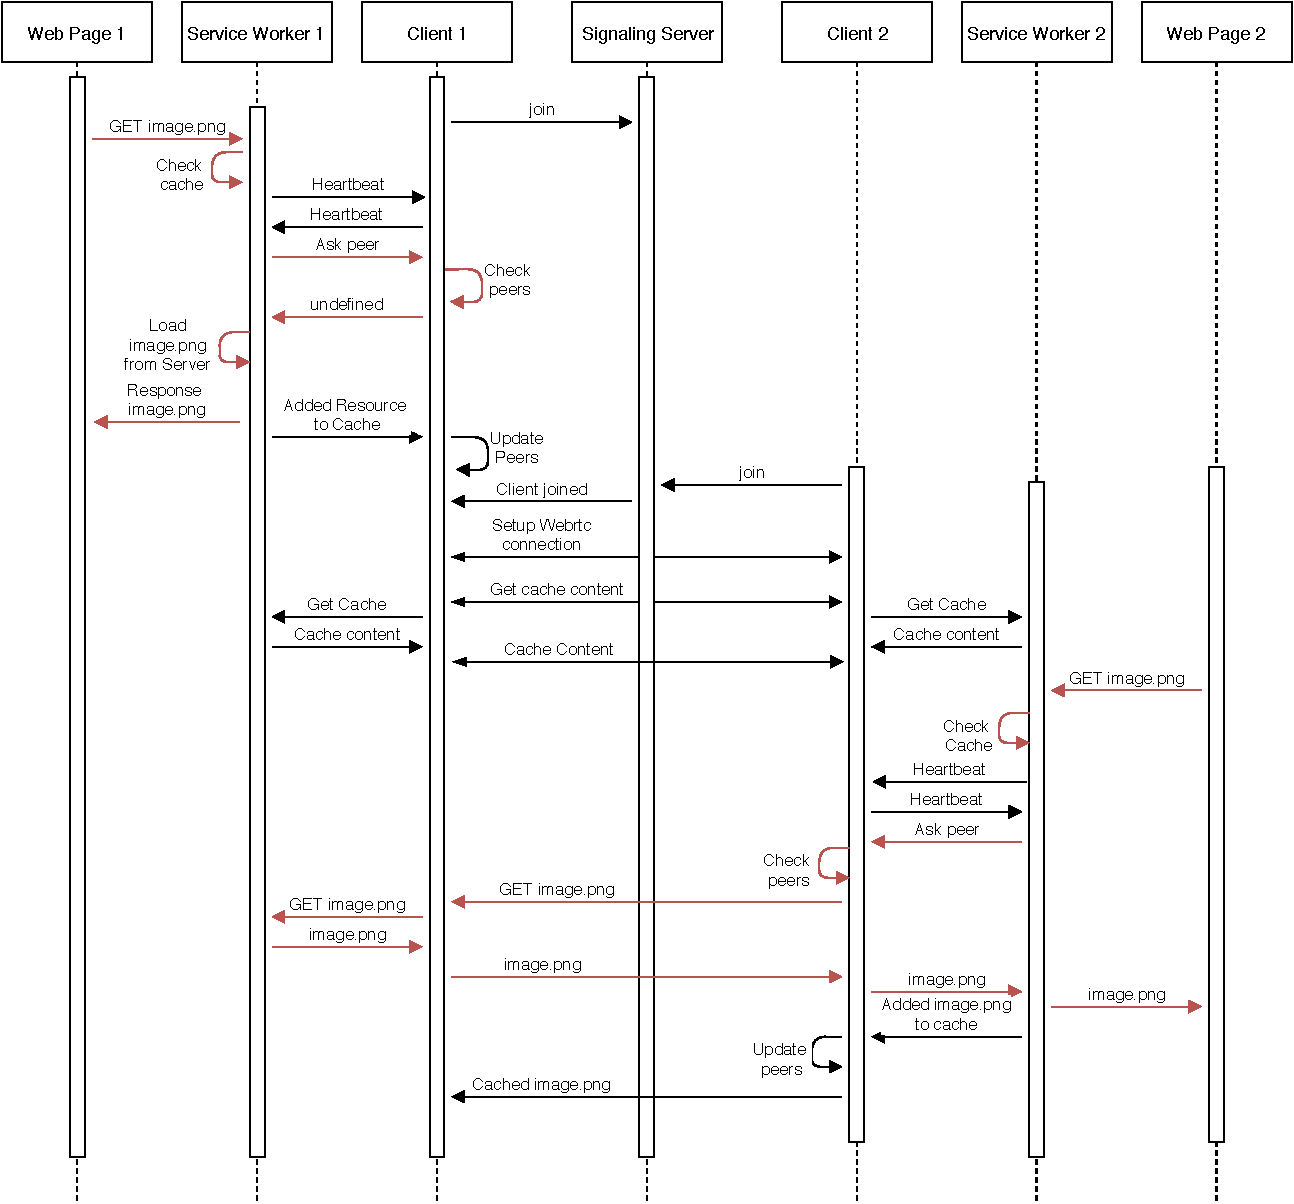
\includegraphics[width=0.8\textwidth]{figures/message_flow_cdn}
	\caption[A Figure Short-Title]{Kommunikationsfluss zwischen zwei Clients um eine Ressource auszutauschen}
	\label{fig:message_flow_cdn}
\end{figure}

Abbildung \ref{fig:message_flow_cdn} zeigt eine vereinfachte Darstellung des Kommunikationsflusses zweier Clients, welche die Ressource img.png laden. Client 1 lädt als erster die Webseite initialisiert das \cdn und meldet sich beim Signaling Server zurück das er dem Peer Mesh beigetreten ist. Die Website versucht anschießend die Ressource img.png zu laden. Diese Anfrage wird vom Service Worker abgefangen, welcher als erstes versucht die Anfrage über seinen eigenen Cache zu beantworten. Da dies nicht möglich ist versucht er nun die Anfrage über das \pTp Netzwerk zu bearbeiten. Dazu muss er das Client Script auffordern bei geeigneten Peers nach der Ressource zu fragen. Da diese Anfrage an die Client blockend ist muss er sich zuerst über einen Heartbeat versichern das das Client Script auch verfügbar ist. Zur Übersichtlichkeit des Diagrams wurde der Heartbeat nicht bei jeder Kommunikation hinzu gefügt. Hat der Service Worker sich vergewissert, dass das Client Script in der Lage ist zu antworten, so sendet er die Anfrage der Ressource image.png an das Client Script. Dieses sucht in der lokalen List von Peers und deren Ressourcen nach einem geeigneten Peer. Dieser ist in diesem Fall nicht vorhanden, weshalb es an den Service Worker undefined sendet. Daraufhin lädt der Service Worker die Ressource über den Server herunter. Anschließend speichert er die Ressource in seinem Cache.

Als nächstes lädt Client 2 die Webseite und teilt dem Signaling Server mit das er dem Peer Mesh beitreten will. Dieser sendet eine Nachricht an Client 1 das ein neuer Peer dem Mesh beigetreten ist. Client 1 initialisiert daraufhin die Webrtc Verbindung zu Client 2. Ist die Verbindung hergestellt tauschen die beiden Clients den Inhalt ihres Caches aus und speichern welche Ressourcen der andere Client gespeichert hat. Nun lädt versucht die Webseite von Client 2 die Ressource image.png zu laden. Der Service Worker von Client 2 fängt die Anfrage ab. Da er die Anfrage nicht mit Hilfe seines Caches beantworten kann beauftragt er Client Script 2 mit der Beantwortung der Anfrage über das \pTp Netzwerk. Client 2 ermittelt Client 1 als geeigneten Peer und sendet die Anfrage der Ressource image.png an Client 1 weiter. Client 1 sendet nun die Anfrage an seinen Service Worker weiter. Dieser lädt die Ressource aus seinem Cachen und leitet sie an Client 1 weiter. Client 1 serialisiert und unterteilt, falls nötig, die Ressource in chunks und sendet sie an Client 2. Client 2 setzt die Antwort nun wieder zusammen deserialisiert sie und sendet die Antwort an seinen Service Worker. Der Service Worker sendet das Response Object an die Webseite und das Bild kann geladen werden.

\subsection{Heartbeats}

Sendet der Service Worker eine Anfrage an das Client Script so muss dieser sicher stellen, das das Script sowohl geladen ist, als auch auf den Service Worker message Channel registriert ist. Zwar ist auch die eigentliche Anfrage an das Client Script mit einem Timeout versehen, jedoch ist dieser deutlich höher als der des Heartbeats. Dieser Heartbeat muss zwischen jeder Kommunikation zwischen Service Worker und Client Script, die blockend ist, durchgeführt werden, da es möglich ist das zwischen der aktuellen und der letzten Anfrage das Client Script beendet wurde oder nicht mehr in der Lage ist auf Anfragen des Service Workers zu reagieren. Gründe dafür können unter anderem sein das ein Fehler geworfen oder das die Seite geschlossen wurde. Wird der Heartbeat weggelassen, so muss im Falle eines nicht antwortenden Scripts immer die maximale Timout Dauer für Anfragen über das \pTp \cdn abgewartet werden. Als Folge würden sich diese Anfragen deutlich verlangsamen.

\subsection{Verbindungsaufbau}
\begin{figure}[!h]
	\centering
	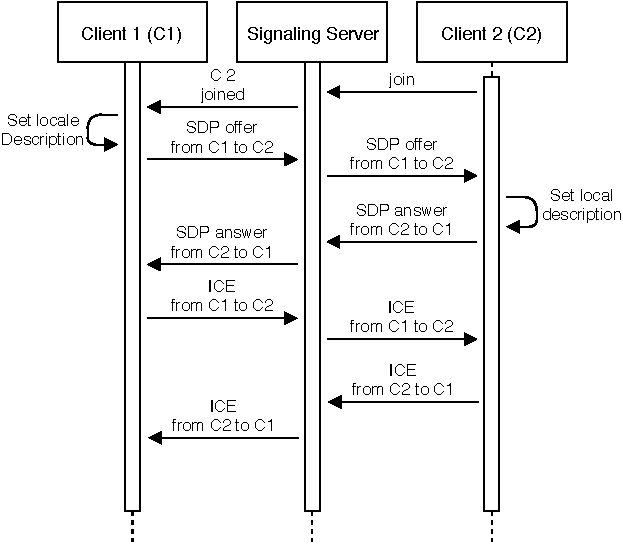
\includegraphics[width=0.8\textwidth]{figures/verbindungsaufbau}
	\caption[A Figure Short-Title]{Flussdiagramm Verbindungsaufbau}
	\label{fig:verbindungsaufbau}
\end{figure}


Tritt ein Client einem Peer Mesh bei so muss er zuerst eine Verbindung zu allen Clients aufbauen die sich bereits im Peer Mesh befinden. Dazu sendet er eine Nachricht an den Signaling Server der diese an alle Peers weiter leitet. Empfängt ein Peer die Nachricht das ein neuer Peer dem Netzwerk beigetreten ist so beginnt er eine Webrtc Verbindung zu dem Peer aufzubauen. Dazu sendet er über den Signaling Server ein SDP Offer an den Peer, der mit einer SDP Answer Nachricht antwortet. Empfängt ein Peer, in \ref{fig:verbindungsaufbau} C1, ein SDP Answer so sende er ein ICE Packet an den Peer von dem er es erhalten hat(C2). Dieser antwortet ebenfalls mit einem ICE Packet und ein DataChannel wird eröffnet. Sämtliche weitere Kommunikation zwischen den beiden Peers wird über den DataChannel gehandhabt. 

\subsection{Cache initialisierung}
\begin{figure}[!h]
	\centering
	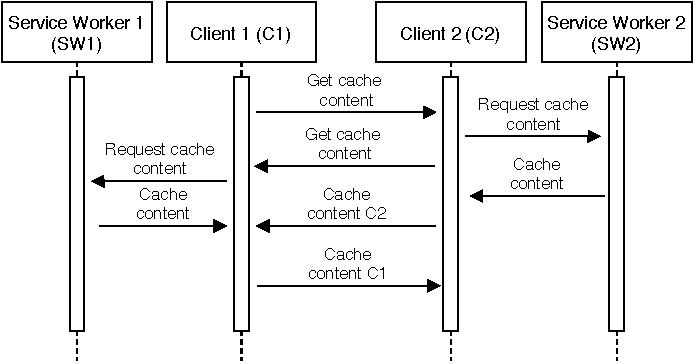
\includegraphics[width=0.8\textwidth]{figures/cache_initialisierung}
	\caption[A Figure Short-Title]{Flussdiagramm Cache Initialisierung}
	\label{fig:cache_initialisierung}
\end{figure}

Nachdem eine \webrtc Verbindung zwischen den Beiden Clients hergestellt ist müssen informationen über den Inhalt der Caches ausgetauscht werden. Dazu senden sich die Clients gegenseitig die Anfrage nach dem Inhalt des Caches. Beide Clients fragen nun ihren Service Worker welche Ressourcen bereits in ihrem Cache vorhanden sind und senden die Liste der zwischengespeicherten Ressourcen an den Client zurück
x
\subsection{Updates}

\begin{figure}[!h]
	\centering
	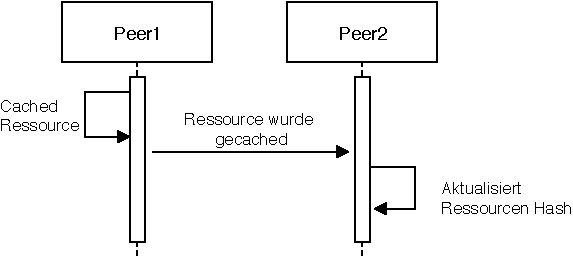
\includegraphics[width=0.8\textwidth]{figures/Ressourcen_update}
	\caption[A Figure Short-Title]{Flussdiagramm Ressourcen Update}
	\label{fig:update_resource}
\end{figure}

Lädt ein Client eine neue Ressource in den Cache oder löscht er eine aus dem Cache so muss er seinem Peer Mesh dies mitteilen. Dazu sendet er eine Nachricht an alle Peers mit denen er verbunden ist. Die Kommunikation findet über den zuvor geöffneten \webrtc DataChannel statt. Empfängt ein Peer ein Update von einem anderen Peer so ändert er entsprechend die gespeicherte Hashmap von Ressourcen für diesen Peer.

Verlässt ein Client das Peer mesh so wird er aus der Liste der verfügbaren Peers gelöscht. Anschließend werden alle offenen Kommunikationen zu dem Peer entfernt. Ein Peer wird als nicht mehr verbunden betrachtet wenn der DataChannel nicht mehr offen ist.


\section{Chunking}
Für den Austausch von Daten werden die von WebRTC angebotene DataChannel genutzt, welche das Stream Control Transmission Protocol kurz SCTP verwendet. Problem hierbei ist, dass dieses Protokoll ursprünglich für die Übertragung von Kontrollinformationen designt wurde und deshalb für die Kompatibilität verschiedener Browser eine Paketgröße von 16kiB nicht überschritten werden sollte. Es ist jedoch notwendig auch größere Dateien zu übertragen, weshalb aktuell viele kleine Datenpakete verwendet werden müssen. Hierdurch entsteht ein nicht zu vernachlässigender Overhead.

\begin{listing}[h]
	\inputminted{javascript}{listings/buffersize.js}
	\caption{Buffersize Berücksichtigung}
	\label{lst:code-buffersize}
\end{listing}
\begin{listing}[h]
	\inputminted{javascript}{listings/handle_chunk.js}
	\caption{Buffersize Berücksichtigung}
	\label{lst:code-handle-chunk}
\end{listing}

Datachannel haben in der aktuellen Browser Implementation eine maximale Buffergröße. Der client der die Datachannel verwendet ist dafür verantwortlich sicher zu stellen, dass die maximale Buffergröße nicht überschritten ist. Ist die maximale Buffergröße erreicht, so werden weitere Chunks erst gesendet, wenn sich der Buffer wieder geleert hat.

Empfängt ein Client eine Anfrage in Form von Chunks so muss er diese wieder zu der eigentlichen Ressource zusammen setzen. Dazu wird für die Anfrage ein Array verwaltet in denen alle empfangenen Chunks gespeichert werden. Wurden alle Chunks einer Anfrage empfangen werden sie wieder zu einem Objekt zusammengesetzt und die Anfrage wird an den Service Worker weiter geleitet

%\begin{itemize}
%	\item evtl serialisierung thematisieren.
%\end{itemize}
%\begin{itemize}
%  \item SCTP(DataChannel) Message size limit 16kiB
%  \item Fixe id länge notwendig
%  \item datachannel buffersize muss berücksichtigt werden
%  \item chunking reassembling nötig
%  \item Performance einbussen
%  \item abToMessage und sendToPeer
%\end{itemize}

% SCTP(DataChannel) message size limit 16kiB
% chunking reassembling nötig
% _abToMessage() und _sendToPeer
% Performance einbußen

%Currently, it is only possible to send messages not larger than 16kiB via the RTCDataChannel. In order to send larger messages chunking and reassembling is necessary. These procedures take place in the _abToMessage() and _sendToPeer() methods in the peer.js file.

%\begin{itemize}
%	\item Details zum Algorithmus
%\end{itemize}
\section{System Test}\label{system-test}
Das Plugin stellt ein Modul bereit um zu testen ob es einem Client möglich ist am \pTp CDN teilzunehmen.

Dazu werden drei Tests bereitgestellt.
\begin{lstlisting}
	p2pCDN.systemTest.testBrowser()
\end{lstlisting}
 Mit Hilfe von modernizr\footnote{https://modernizr.com/} testet die Funktion ob die verwendete Browserversion alle benötigten Funktionen unterstützt. Modernizr ist eine Javascript Bibliothek mit der getestet werden kann ob ein Browser bestimmte Funktionen unterstützt.
\begin{lstlisting}
	p2pCDN.systemTest.webrtcInitialized()
\end{lstlisting}
Gibt ein Promise zurück welches überprüft ob die webrtc Verbindung erfolgreich aufgebaut wurde. Da die Initialisierung einen Moment in Anspruch nehmen kann wird wiederholt geprüft ob die Verbindung aufgebaut wurde.
\begin{lstlisting}
	p2pCDN.systemTest.clientConnected()
\end{lstlisting}
Gibt ebenfalls ein Promise zurück und überprüft ob erfolgreich eine Verbindung zu einem anderen Client aufgebaut werden konnte. Um diesen Test erfolgreich auszuführen muss sich ein andere Client im aktuellen Peer mesh befinden.

\section{Erfassen von Statistiken}\label{ch:implementation:stats}
\begin{listing}[h]
	\inputminted{javascript}{listings/sendStatistic.js}
	\caption{Erfassen der Statistiken}
	\label{lst:code-stats}
\end{listing}
\begin{listing}[h]
	\inputminted{javascript}{listings/logStatistic.js}
	\caption{Erfassen der Statistiken}
	\label{lst:code-stats}
\end{listing}

\begin{listing}[h]
	\inputminted{javascript}{listings/_handle_chunk.js}
	\caption{}
	\label{lst:handle_chunk}
\end{listing}

\begin{listing}[h]
	\inputminted{javascript}{listings/handle_request.js}
	\caption{Abarbeitung eines Request im Service Worker}
	\label{lst:handle_request}
\end{listing}

Um die Nutzungsstatistiken des CDNs zu erfassen sendet jeder Client periodisch POST requests an den Server. Dazu sammelt der Service Worker alle Anfragen die in einem Zeitraum von 10 Sekunden angefallen sind und sendet sie gebündelt als JSON an den Server.

Erfasst werden:
\begin{description}
\item[peerId]\hfill \\
Die PeerId bezeichnet die Id des peers der die Statistik sendet.
\item[method]\hfill \\
Method gibt an wie die Anfrage behandelt wurde und kann die Werte 'cacheResponse', 'peerResponse' oder 'serverResponse' beinhalten. Ein cacheResponse konnte aus dem eigenen Cache beantwortet werden. ServerResponse bedeutet das die Anfrage über den externen Server geladen werden musste. Der Wert peerResponse gibt an das die Anfrage über das \pTp CDN bearbeitet werden konnte.
\item[from]\hfill \\
 'From' gibt an woher die Anfrage geladen wurde. Im Falle eines serverResponses beinhaltet sie den Wert 'server' und bei einem cacheResponse den Wert cache. Wurde die Anfrage über das \pTp Netzwerk beantwortet beinhaltet sie die peerId des Peers der die Anfrage beantwortet hat. Dazu sendet das Script neben der eigentlichen Anfrage auch die eigene PeerId und die PeerId des peers der die Anfrage beantwortet hat an die Service Worker. (siehe \ref{lst:handle_chunk}) 
\item[URL]\hfill \\
Die URL enthält die URL der angefragten Ressource. 
\item[timing]\hfill \\
Timing beinhaltet die Zeitspanne die benötigt wurde um die Anfrage zu beantworten, beginnend vor der Entscheidung wie der Request abgearbeitet werden soll(siehe \ref{lst:handle_request}) und endend nach dem die Anfrage empfangen wurde. Nicht enthalten in der Zeitspanne ist die Entscheidung ob der Service worker den Request bearbeitet und die Renderzeiten des Browsers. Diese Zeiten sind nicht abhängig von der Art der Request Beantwortung.(siehe Evaluation)
\end{description}
Mit Hilfe der Configuration kann festgelegt werden an welchen Endpunkt die Statistik gesendet werden soll. Die Anwendung ist für das speichern und verarbeiten der Daten zuständig, dies ist nicht Teil des Plugins. Slidesync speichert die Daten als JSON in Redis und stellt einen JSON Endpunkt zur Verfügung mit dem die Statistiken abgerufen werden können. Für die Labortests werden die Daten in JSON Dateien zur späteren Verarbeitung abgelegt.


%\begin{itemize}
%	\item 	evtl. Mongo db
%	\item 	anzeigetool
%	\item schoolcloud
%\end{itemize}

\section{Quota limits - Löschen von Requests aus dem Cache}
\begin{table}[!htb]
	\begin{center}


	\begin{tabular}{|r|l|l|}
		\hline
		Browser	 & Limit \\ \hline
		Chrome & < 6\% des freien Fesplattenspeichers \\ \hline
		Firefox & < 10\% des freien Fesplattenspeichers \\ \hline
		Safari & < 50MB \\ \hline
		IE10 & < 250MB \\ \hline
		Edge & Abhännig von der Festplattengröße \\ 
		\hline
	\end{tabular}
	\caption{Browser Storage Quotas\cite{offline-pwa}}

\end{center}
\end{table}

Browser stellen den Clients unterschiedlich viel Speicherplatz für offline Caches zur Verfügung. Ist das Quota limit erreicht versuchen Firefox und Chrome Speicher frei zu machen indem Elemente aus dem Cache gelöscht werden. Dabei werden jedoch keine einzelnen Elemente aus dem Cache gelöscht sondern mittels Last-recently-used(LRU) werden ganze Caches gelöscht. Safari und Edge haben keinen Mechanismus zum automatischen Löschen von Elementen sondern werfen lediglich einen Fehler.\cite{offline-pwa} Deshalb ist es notwendig das der Service Worker in dem Fall das das Limit erreicht wird Elemente löscht.

Mit Hilfe der Quota Management API\cite{quota-api-ff} ist es möglich die momentane Speichernutzung auszulesen ebenso wie den maximal Verfügbaren Speicherplatz. Ist diese Limit oder das Quota Limit welches über die Konfiguration angegeben wurde erreicht, löscht der Service Worker so lange die ältesten Einträge im Cache, bis genügend Speicher für den nächsten Request vorhanden ist. Dazu berechnet der Service Worker die Größe des zu speichernden Request. 

%	\item https://developers.google.com/web/updates/2017/08/estimating-available-storage-space
%	\item https://developer.mozilla.org/en-US/docs/Web/API/IndexedDB_API/Browser_storage_limits_and_eviction_criteria

%\section{Resource loading}

\section{Tests}
Um das Plugin zu testen wird als test Runner Karma verwendet.\footnote{https://karma-runner.github.io/latest/index.html} Als test framework wird mochajs\footnote{https://mochajs.org/} und als assertion Library wird Chai\footnote{https://www.chaijs.com/} eingesetzt 

%- mocha
%- chai
%- karma
% Event handler testen
% 	- registrieren/abmelden --> test helper

%\section{Ressourcen Management}

\section{Configuration}
\begin{listing}[h]
	\inputminted{javascript}{listings/configuration.js}
	\caption{Beispielhafte Konfiguration}
	\label{lst:configuration}
\end{listing}

Um eine gute Anpassung an verschiedene Anwendungsfälle zu ermöglichen bietet das \pTp CDN eine Reihe von Konfigurationsmöglichkeiten. Nachdem das Client Script die Konfiguration geladen hat wird sie im der Indexed DB gespeichert und von dort durch den Service Worker geladen.\ref{lst:configuration} zeigt eine Beispielhaft Konfiguration des CDNs im Folgenden werden die verschiedenen Konfigurationsmöglichkeiten aufgelistet und beschrieben.

\begin{description}
\item[channel]\hfill \\
Bezeichnet den für das Peer Meshing zu verwendenden Websocket channel. Alle Clients mit dem selben Channel befinden sich im selben Peer Mesh.
\item[clientId]\hfill \\
Eindeutiger Identifizier mit dem der Peer identifiziert werden kann. Ähnlich einer Session ID wird er verwendet um Clients wieder zuerkennen und anzusprechen.
\item[idLength]\hfill \\
Bezeichnet die maximale Länge der ClientIds. Kürzere ClientIds werden bis zu dieser Länge aufgefüllt. Wird benötigt um intern bei dem verschicken von Paketen über das CDN ClientIds fester länge verwenden zu können.(siehe \todo{referenzieren}) 
\item[stunServer]\hfill \\
Gibt den zu verwendenden STUN Server an. Dies kann ein öffentlicher oder privat betriebener Server sein. Kann freigelassen werden falls kein STUN Server verwendet werden soll
\item[verbose]\hfill \\
Aktiviert/deaktiviert Debug Ausgaben.
\item[serviceWorker]\hfill \\
Beinhaltet alle Konfigurationen die den Service Worker betreffen.
\item[urlsToShare]\hfill \\
Liste aller URL die mit Hilfe des CDN bearbeitet werden sollen. Urls können als Regex definiert werden.
\item[excludedUrls]\hfill \\
Liste von URLs die explizit von dem CDN ausgeschlossen werden sollen. Ebenso wie urlsToShare werden excludedUrls als Regex interpretiert.
\item[path]\hfill \\ und Text dahinter
Pfad von dem das Service Worker Script geladen werden soll.
\item[scope]\hfill \\
Gibt den Scope an unter dem der Service Worker arbeiten soll. 
\item[basePath]\hfill \\
Gibt den Service Worker Base Path an.
\item[storageQuota]\hfill \\
Maximal für das CDN zu verwendender Cache Speicher. Überschreitet der Cache den Wert, werden so lange Ressourcen aus dem Cache gelöscht bis der Wert unterschritten ist. (siehe \todo{ref}) 
\item[cachingEnabled]\hfill \\
Aktiviert/Deaktiviert das Caching innerhalb des Service Workers. Nützlich zum Debuggen.
\item[verbose]\hfill \\
Gibt an ob der Service Worker debugging Ausgaben auf die Konsole schreiben soll.
\item[statisticPath]\hfill \\
URL an die die erhobenen Statistiken gesendet werden sollen. siehe \ref{ch:implementation:stats}

\end{description}


%\section{Reusability}

\section{Netzwerk Konfiguration}

Um eine fehlerfreie Funktion des \cdns zu gewährleisten muss sichergestellt sein das sich die Clients miteinander verbinden können. Inbesondere in Unternehmensnetzwerken kann dies ein Problem darstellen. Häufig sind in diesen Netzwerken strenge Firewall regeln aktiv die nur die Kommunikation über bestimmte Ports erlauben. Da Webrtc eine relativ große range an Ports verwendet, aus der zufällig ein freier ausgewählt wird ist es nicht immer eine Option alle Ports explicit zu öffnen. Wird eine Firewall verwendet die nur den ein und ausgehenden Datenverkehr überwacht, so können weiterhin Verbindungen innerhalb des lokalen Netzwerkes hergestellt werden. Das im Rahmen dieser Arbeit vorgestellte \cdn ist damit weiterhin in der Lage Inhalte unter den Nutzern zu verteilen. Ein größeres Problem stellen hier Client seitige Firewalls dar. Zwar könnte theoretisch der Datenverkehr über TURN Server geleitet werden, jedoch wird in diesem Fall der gesamte Verkehr über einen Server geleitet der sich unter Umständen nicht im selben lokalen Netzwerk befindet. Das \cdn ist in diesem Fall nicht in der Lage die Belastung des Netzwerkes zu reduzieren. In diesem Fall bleibt nur die Möglichkeit die verwendeten Ports Clientseitig zu öffnen. Chrome bietet die Möglichkeit die für \webrtc verwendeten Ports einzustellen.\cite{chrome-port-range} 

Soll eine Kommunikation zwischen Nutzern möglich sein die sich nicht im selben lokalen Netzwerk befinden, so muss in den meisten Netzwerken aufgrund von NAT ein STUN Server spezifiziert werden.  
